%%%%%%%%%%%%%%%%%%%%%%%%%%%%%%%%%%%%%%%%%%%%%%%%%%%%%%%%%%%%%%%%%%%%%%%%%%%%%%%%
%2345678901234567890123456789012345678901234567890123456789012345678901234567890
%        1         2         3         4         5         6         7         8

\documentclass[letterpaper, 10 pt, conference ,onecolumn]{ieeeconf}  % Comment this line out if you need a4paper


%\documentclass[•]{•}4paper, 10pt, conference]{ieeeconf}      % Use this line for a4 paper

\IEEEoverridecommandlockouts                              % This command is only needed if 
                                                          % you want to use the \thanks command

\overrideIEEEmargins                                      % Needed to meet printer requirements.

% See the \addtolength command later in the file to balance the column lengths
% on the last page of the document

% The following packages can be found on http:\\www.ctan.org
\usepackage{graphics} % for pdf, bitmapped graphics files
%\usepackage{epsfig} % for postscript graphics files
%\usepackage{mathptmx} % assumes new font selection scheme installed
%\usepackage{times} % assumes new font selection scheme installed
%\usepackage{amsmath} % assumes amsmath package installed
%\usepackage{amssymb}  % assumes amsmath package installed

%-----------------------------------------------------------------------------
% Correct bad hyphenation here
%-----------------------------------------------------------------------------
\hyphenation{op-tical net-works semi-conduc-tor}

%-----------------------------------------------------------------------------
% Graphics 
%-----------------------------------------------------------------------------
\usepackage{graphicx}
%\usepackage{caption}
%\usepackage{subfigure}
%\usepackage{subfloat}

\usepackage[tight,footnotesize]{subfigure}
	

%-----------------------------------------------------------------------------
% Orange notes 
%-----------------------------------------------------------------------------
\usepackage{todonotes}

%-----------------------------------------------------------------------------
% Hidden comments
%-----------------------------------------------------------------------------
\usepackage{comment}

%-----------------------------------------------------------------------------
% footnote
%-----------------------------------------------------------------------------
\usepackage{footnote}

%-----------------------------------------------------------------------------
% Acronyms  
%-----------------------------------------------------------------------------
\usepackage[nolist]{acronym}


%-----------------------------------------------------------------------------
% In-text author's citation  
%-----------------------------------------------------------------------------

%-----------------------------------------------------------------------------
% Strikethrough  
%-----------------------------------------------------------------------------
\usepackage{soul}

%-----------------------------------------------------------------------------
% Math
%-----------------------------------------------------------------------------
\usepackage{amsmath}
\usepackage{amsfonts}

%-----------------------------------------------------------------------------
% Set the default folder for images
%-----------------------------------------------------------------------------
\graphicspath{{images/}} 

%-----------------------------------------------------------------------------
% References
%-----------------------------------------------------------------------------
\usepackage{hyperref}

\usepackage{color} 
\definecolor{keywords}{RGB}{255,0,90}
\definecolor{comments}{RGB}{0,0,113}
\definecolor{red}{RGB}{160,0,0}
\definecolor{green}{RGB}{0,150,0}
\definecolor{blue}{rgb}{0.0, 0.0, 0.99}	
\definecolor{black}{rgb}{0.0, 0.0, 0.0}	
\definecolor{backcolour}{rgb}{0.95,0.95,0.92}


\usepackage[procnames]{listings}

\usepackage{caption}

\definecolor{keywords}{RGB}{255,0,90}
\definecolor{comments}{RGB}{0,0,113}
\definecolor{red}{RGB}{160,0,0}
\definecolor{green}{RGB}{0,150,0}
\definecolor{black}{rgb}{0.0, 0.0, 0.0}	
\definecolor{backcolour}{rgb}{0.95,0.95,0.92}


\usepackage[procnames]{listings}

\usepackage{caption}

\lstset{language=Python, 
        basicstyle=\ttfamily\footnotesize, 
        backgroundcolor=\color{backcolour}, 
        keywordstyle=\color{keywords}\ttfamily,
        commentstyle=\color{green}\ttfamily,
        stringstyle=\color{red}\ttfamily, 
        identifierstyle=\color{black}\ttfamily,
        procnamekeys={def,class} ,
	stepnumber=1, 
  	numbersep=10pt,                        
  	tabsize=2,                            
  	extendedchars=true,                     
  	breaklines=true,                 
  	captionpos=t,                          
  	mathescape=true,
  	showspaces=false,  
  	showtabs=false,           
  	xleftmargin=17pt,
  	framexleftmargin=17pt,
  	framexrightmargin=17pt,
  	framexbottommargin=5pt,
  	framextopmargin=5pt,
  	showstringspaces=false }
        
\DeclareCaptionFormat{listing}{\rule{\dimexpr\textwidth+17pt\relax}{0.4pt}\par\vskip1pt#1#2#3}
\captionsetup[lstlisting]{format=listing,singlelinecheck=false, margin=0pt,labelsep=space,labelfont=bf}

\renewcommand\lstlistingname{Implementation}




  
\makeatletter
\def\BState{\State\hskip-\ALG@thistlm}
\makeatother

\hypersetup{
	colorlinks = true, 
	breaklinks = true, 
	bookmarks = true,
	bookmarksnumbered,
	urlcolor = blue, 
	linkcolor = blue, 
	citecolor = blue, 
	linktoc=page, 
	pdftitle={}, 
	pdfauthor={\textcopyright Author}, 
	pdfsubject={}, 
	pdfkeywords={}, 
	pdfcreator={pdfLaTeX}, % PDF Creator
	pdfproducer={IEEE} 
}

\title{
Computer Vision Assignment 2
}

%-----------------------------------------------------------------------------
%\begin{acronym}
 
%\end{acronym}

\author{
 Asem Abdelaziz,
 Mohamed Abdallah, 
 Taha Ali,
 Abdelrahman Sayed
}

\begin{document}

\maketitle



\section{Problem1: Hough Transform} 
\subsection{Line Detection} 


The general overview of line detection routine using \textit{Hough Transform}:
\begin{enumerate}

\item Edge detection (eg. using \textit{Canny edge detector}).
\item Mapping each edge point to the \textit{Hough space}.
\item For each mapped point, vote for each candidate line passing through the point, by incrementing an accumulator array at the corresponding line; line is represented by $\theta$ and $\rho$ (i.e angle and distance, respectively).
\item Extract the most candidate lines.

\end{enumerate} 
\subsection*{Implementation}

\textit{Python} is used as a wrapper to perform matrix operations to perform edge detection and lines detection. \textit{OpenCV} is only used for verifying our results, loading/showing images, and drawing lines.


\subsection*{Canny Edge Detection: Implementation} 
The snippet code provided in ~\nameref{imp:canny-main} shows the workflow of \textit{Canny edge detector}, the details of the invoked subroutines are provided in the ~\nameref{imp:canny-all}.

\subsection*{Hough Lines Detection: Implementation }


Note that mathematical library \textit{numpy} is the only dependency in our implementation in \textit{python}. see ~\nameref{imp:hough-lines}.

\subsection*{Results}
Using our implementation we could produce the following images. see Figure ~\ref{fig:houghlines-origianl}, ~\ref{fig:houghlines-canny}, ~\ref{fig:houghlines-linesonly}, ~\ref{fig:houghlines-lines-and-canny}, and ~\ref{fig:houghlines-final}.
\begin{figure}[h!]
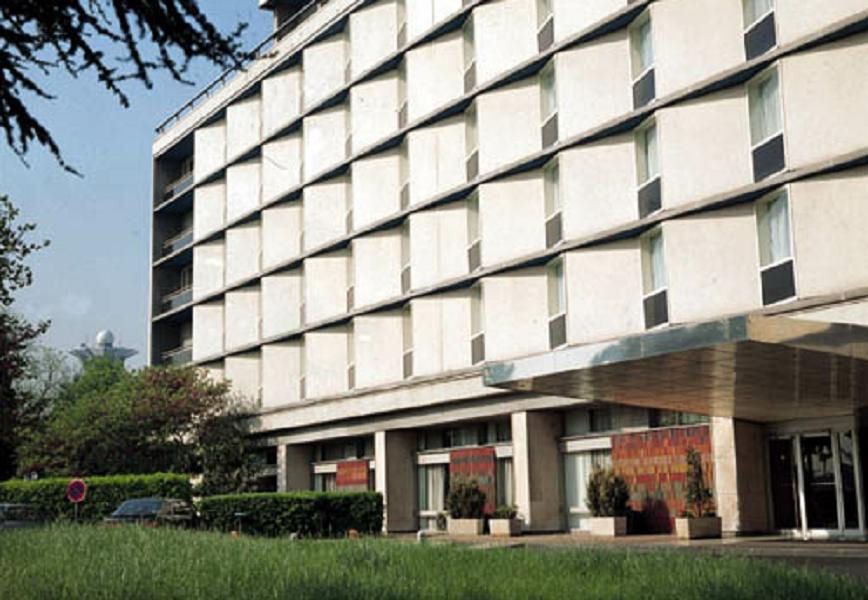
\includegraphics[width=0.4\paperwidth]{hough-lines/lines.jpg}
\caption{Original image of interest.}
\label{fig:houghlines-origianl}
\end{figure}

\begin{figure}[h!]
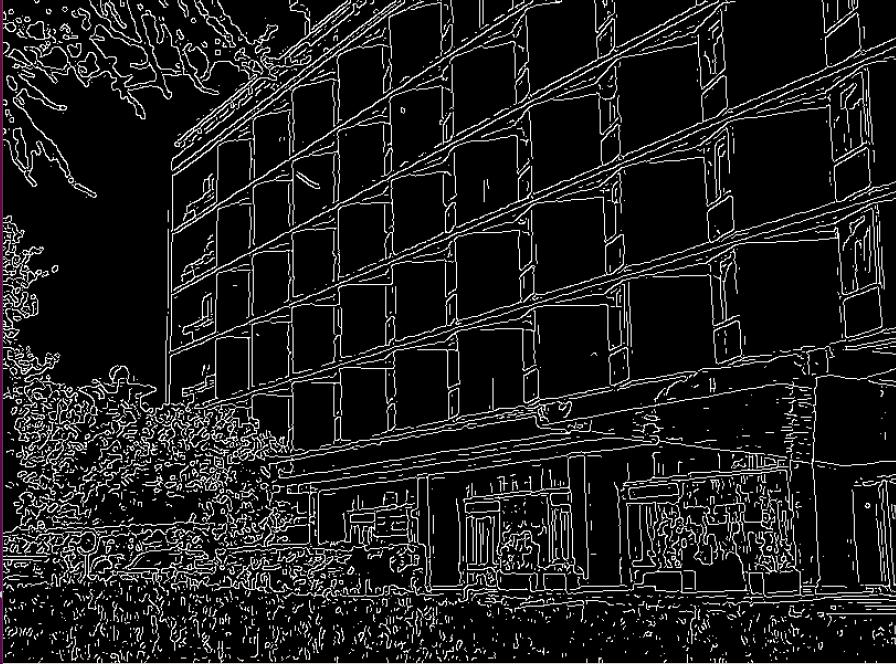
\includegraphics[width=0.4\paperwidth]{hough-lines/canny-image.jpg}
\caption{Edge detection using \textit{canny algorithm} in ~\nameref{imp:canny-main}}
\label{fig:houghlines-canny}
\end{figure}

\begin{figure}[h!]
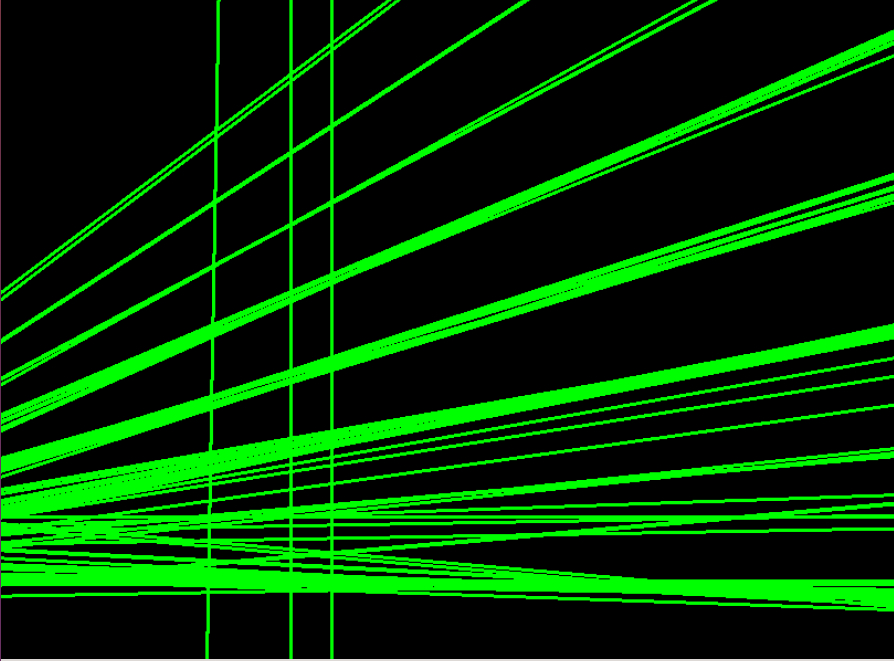
\includegraphics[width=0.4\paperwidth]{hough-lines/linesonly-image.jpg}
\caption{Lines detection using \textit{Hough Algorithm} in ~\nameref{imp:hough-lines}}
\label{fig:houghlines-linesonly}
\end{figure}

\begin{figure}[h!]
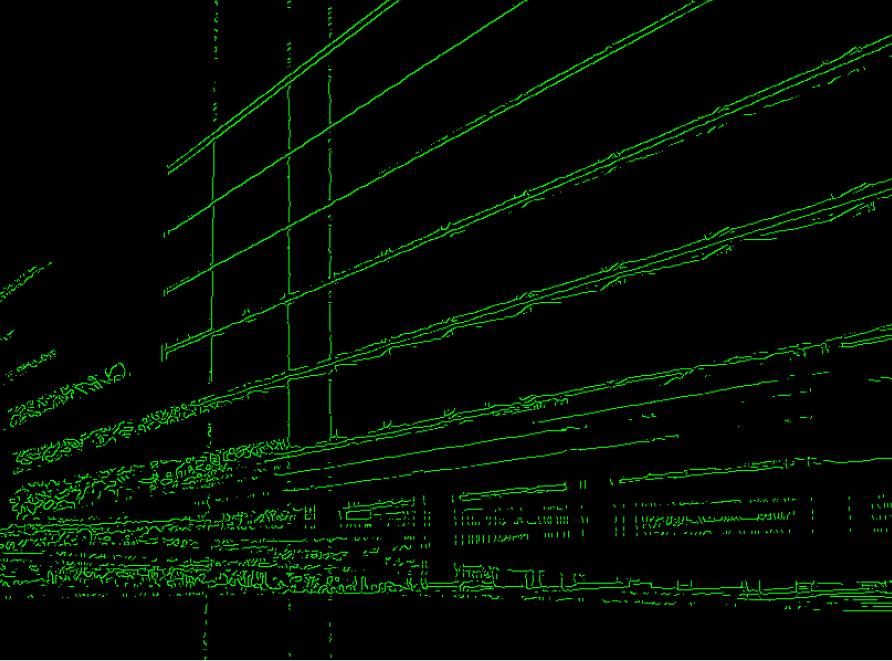
\includegraphics[width=0.4\paperwidth]{hough-lines/lines-AND-canny-image.jpg}
\caption{After performing bitwise AND operation between image in Figure ~\ref{fig:houghlines-canny} and image in Figure ~\ref{fig:houghlines-linesonly} to vanish excessive lines.}
\label{fig:houghlines-lines-and-canny}
\end{figure}

\begin{figure}[h!]
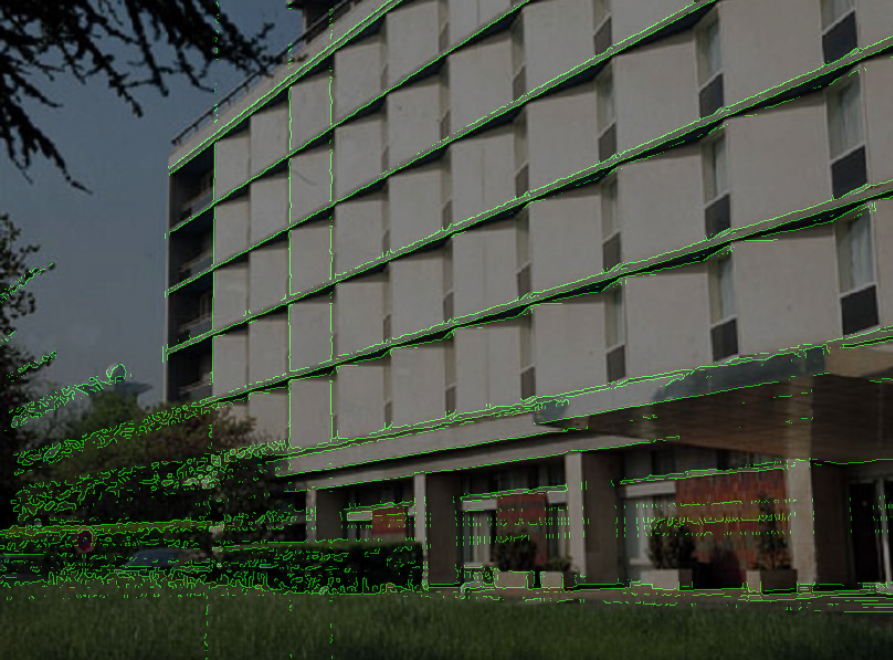
\includegraphics[width=0.4\paperwidth]{hough-lines/final-image.jpg}
\caption{Final image after superimposing lines in Figure ~\ref{fig:houghlines-lines-and-canny} on the original image in ~\ref{fig:houghlines-origianl}. }
\label{fig:houghlines-final}
\end{figure}

\newpage
\subsection{ Hough Circles Detection }



\newpage

\section*{Problem2: Active Contour Model}
%----------------------------------------------------------------------------------------
%	BIBLIOGRAPHY
%----------------------------------------------------------------------------------------
\bibliographystyle{IEEEtran}
\bibliography{references.bib} % The file containing the bibliography

\section*{Appendix }

\begin{lstlisting}
def myCanny( image , ksize , sigma , minThreshold , maxThreshold ) :
    # 1.Guassian Blurring.
    smoothedImage = __cannySmoothing__(image , ksize , sigma)

    # 2.Gradient and Phase Image based on Sobel edge detection.
    gradientImage , phaseImage = __cannyEdgeDetection__(smoothedImage , ksize)

    # 3.Non-Maximum Supression for thinning edges.
    nmsImage = __cannyNonMaximumSupression__(gradientImage , phaseImage)

    # 4.Double Thresholding.
    doubleThresholdedImage = __cannyDoubleThresholding__(nmsImage ,
                                                         minThreshold ,
                                                         maxThreshold)

    # 5.Edge Tracking by Hysterysis.
    edgeTrackedImage = __cannyEdgeTracking__(doubleThresholdedImage ,
                                             maxThreshold ,
                                             minThreshold)

    return edgeTrackedImage
\end{lstlisting}


\begin{lstlisting}
import numpy as np


def frange( initial , final , step ) :
    while initial < final :
        yield initial
        initial += step


def __extractLines__( accumulator , angles , threshold ) :
    lines = []
    for angle_index in range(accumulator.shape[0]) :
        for rho in range(accumulator.shape[1]) :
            if accumulator[angle_index , rho] > threshold :
                angle = angles[angle_index]
                # print (angle , rho , accumulator[angle_index , rho])
                lines.append((angle , rho))

    return lines


def myHoughLines( binaryImage , angleAccuracy , threshold ) :
    angles = frange(0 , np.pi , angleAccuracy)
    angles = np.fromiter(angles , dtype = np.float16)

    cartesianWidth = binaryImage.shape[1]
    cartesianHeight = binaryImage.shape[0]

    maxRadius = np.sqrt(cartesianWidth * cartesianWidth +
                        cartesianHeight * cartesianHeight)

    polarWidth = 180  # 180 degree
    polarHeight = int(maxRadius + 0.5)

    # Construct the empty accumulator
    accumulator = np.zeros((polarWidth , polarHeight) , dtype = np.uint16)
    print "Accumulator size:"
    print accumulator.shape
    # Caculate all sines and cosines once to reduce the overhead of redundant
    # float operations.
    sine_table = np.sin(angles , dtype = np.float16)
    cosine_table = np.cos(angles , dtype = np.float16)

    print "Extracting edge points"
    edge_points = [(row , col) for row in range(binaryImage.shape[0]) for col in
                   range(binaryImage.shape[1]) if binaryImage[row , col] != 0]

    edge_points = np.asanyarray(edge_points , dtype = np.uint16)

    for angle_index in range(polarWidth) :
        rho = np.array(np.round(sine_table[angle_index] * edge_points[: , 0] + \
                                cosine_table[angle_index] * edge_points[: ,
                                                            1]) , dtype = int)

        for r in np.nditer(rho , op_flags = ['readonly']) :
            accumulator[angle_index , r] += 1

    lines = __extractLines__(accumulator , angles , threshold)
    print("lines count:")
    print len(lines)
    # print lines
    return lines

\end{lstlisting}


\begin{lstlisting}[caption=Python implementation for Hough Lines Detection,label=imp:hough-lines]
import numpy as np


def frange( initial , final , step ) :
    while initial < final :
        yield initial
        initial += step


def __extractLines__( accumulator , angles , threshold ) :
    lines = []
    for angle_index in range(accumulator.shape[0]) :
        for rho in range(accumulator.shape[1]) :
            if accumulator[angle_index , rho] > threshold :
                angle = angles[angle_index]
                # print (angle , rho , accumulator[angle_index , rho])
                lines.append((angle , rho))

    return lines


def myHoughLines( binaryImage , angleAccuracy , threshold ) :
    angles = frange(0 , np.pi , angleAccuracy)
    angles = np.fromiter(angles , dtype = np.float16)

    cartesianWidth = binaryImage.shape[1]
    cartesianHeight = binaryImage.shape[0]

    maxRadius = np.sqrt(cartesianWidth * cartesianWidth +
                        cartesianHeight * cartesianHeight)

    polarWidth = 180  # 180 degree
    polarHeight = int(maxRadius + 0.5)

    # Construct the empty accumulator
    accumulator = np.zeros((polarWidth , polarHeight) , dtype = np.uint16)
    print "Accumulator size:"
    print accumulator.shape
    # Caculate all sines and cosines once to reduce the overhead of redundant
    # float operations.
    sine_table = np.sin(angles , dtype = np.float16)
    cosine_table = np.cos(angles , dtype = np.float16)

    print "Extracting edge points"
    edge_points = [(row , col) for row in range(binaryImage.shape[0]) for col in
                   range(binaryImage.shape[1]) if binaryImage[row , col] != 0]

    edge_points = np.asanyarray(edge_points , dtype = np.uint16)

    for angle_index in range(polarWidth) :
        rho = np.array(np.round(sine_table[angle_index] * edge_points[: , 0] + \
                                cosine_table[angle_index] * edge_points[: ,
                                                            1]) , dtype = int)

        for r in np.nditer(rho , op_flags = ['readonly']) :
            accumulator[angle_index , r] += 1

    lines = __extractLines__(accumulator , angles , threshold)
    print("lines count:")
    print len(lines)
    # print lines
    return lines
\end{lstlisting}


\begin{lstlisting}[caption=Python implementation for Hough Circles Detection , label=imp:hough-circles]
import numpy as np
def myHoughCircles( binaryImage , threshold ) :
    maxRadius = int(np.sqrt(2)*max(binaryImage.shape)  )
    cartesianWidth = binaryImage.shape[ 1 ]
    cartesianHeight = binaryImage.shape[ 0 ]

    accumulator = np.ndarray((cartesianHeight , cartesianWidth , maxRadius) ,
                             dtype = int )
    accumulator.fill(0)

    print "Extracting edge points"
    edge_points = [ (row , col) for row in range(binaryImage.shape[ 0 ]) for col
                    in range(binaryImage.shape[ 1 ]) if
                    binaryImage[ row , col ] != 0 ]

    edge_points = np.asanyarray(edge_points , dtype = np.uint16)

    print "Accumulation"
    for row in range(accumulator.shape[ 0 ]) :
        for col in range(accumulator.shape[ 1 ]) :
            radius = np.round(np.sqrt(np.square(edge_points[ : , 0 ] - row) +
                                      np.square(edge_points[ : , 1 ] - col)))
            radius = radius.astype(dtype = int , copy = False)

            radius , count = np.unique(radius , return_counts = True)
            # count = count.astype(dtype = np.uint16 , copy = False)
            accumulator[ row , col , radius ] += count


    print "Max circle"
    print np.amax(accumulator)
    print "Extract most candidate circles"
    circles = np.where(accumulator > threshold)
    circles = np.transpose(circles)
    circles = tuple(map(tuple , circles))
    circles = [ (col , row , r) for row , col , r in circles ]

    return circles
\end{lstlisting}


\end{document}

